\documentclass[nonav,sleutel,handout]{beamer}
\usepackage[utf8]{inputenc}
\usepackage[T1]{fontenc}
\title{Politicians and Nobel Prizes}
\date[ISPN '80]{Prof. Dr. Bettina Berendt\\ Knowledge \& the Web 2015-2016}
\author{Katrien Laenen \and Gust Verbruggen \and Ward Schodts}

\usetheme{kuleuvenstijl}

\usepackage{float}
\usepackage{graphicx}
\usepackage{caption}
\usepackage{subcaption}
\graphicspath{ {images/} }




\begin{document}


%%%%%%%%%%%%%%%%%%%%%%%%%%%%%%%%%%%%%%%%%%%%%%%%%%%%%%%%%%%%%%%%%%%%%%%%%%%%%%%%%%%%%%%%%%%%%%%

\begin{frame}
\titlepage
\end{frame}

%%%%%%%%%%%%%%%%%%%%%%%%%%%%%%%%%%%%%%%%%%%%%%%%%%%%%%%%%%%%%%%%%%%%%%%%%%%%%%%%%%%%%%%%%%%%%%%

\begin{frame}[noframenumbering]
\frametitle{Outline} 
  \tableofcontents[hideallsubsections
  ]

\end{frame}

\AtBeginSection[]
{
 \begin{frame}<beamer>
 \frametitle{Outline}
 \tableofcontents[hideothersubsections,currentsection]
 \end{frame}
}


%%%%%%%%%%%%%%%%%%%%%%%%%%%%%%%%%%%%%%%%%%%%%%%%%%%%%%%%%%%%%%%%%%%%%%%%%%%%%%%%%%%%%%%%%%%%%%%
\section{Introduction}
\subsection{Some history}
\begin{frame}
\frametitle{Some history}
\framesubtitle{Nobelprizes, what are they?}
\begin{center}


\begin{figure}[H]
    
    \hfill
    \begin{subfigure}[b]{0.33\textwidth}
        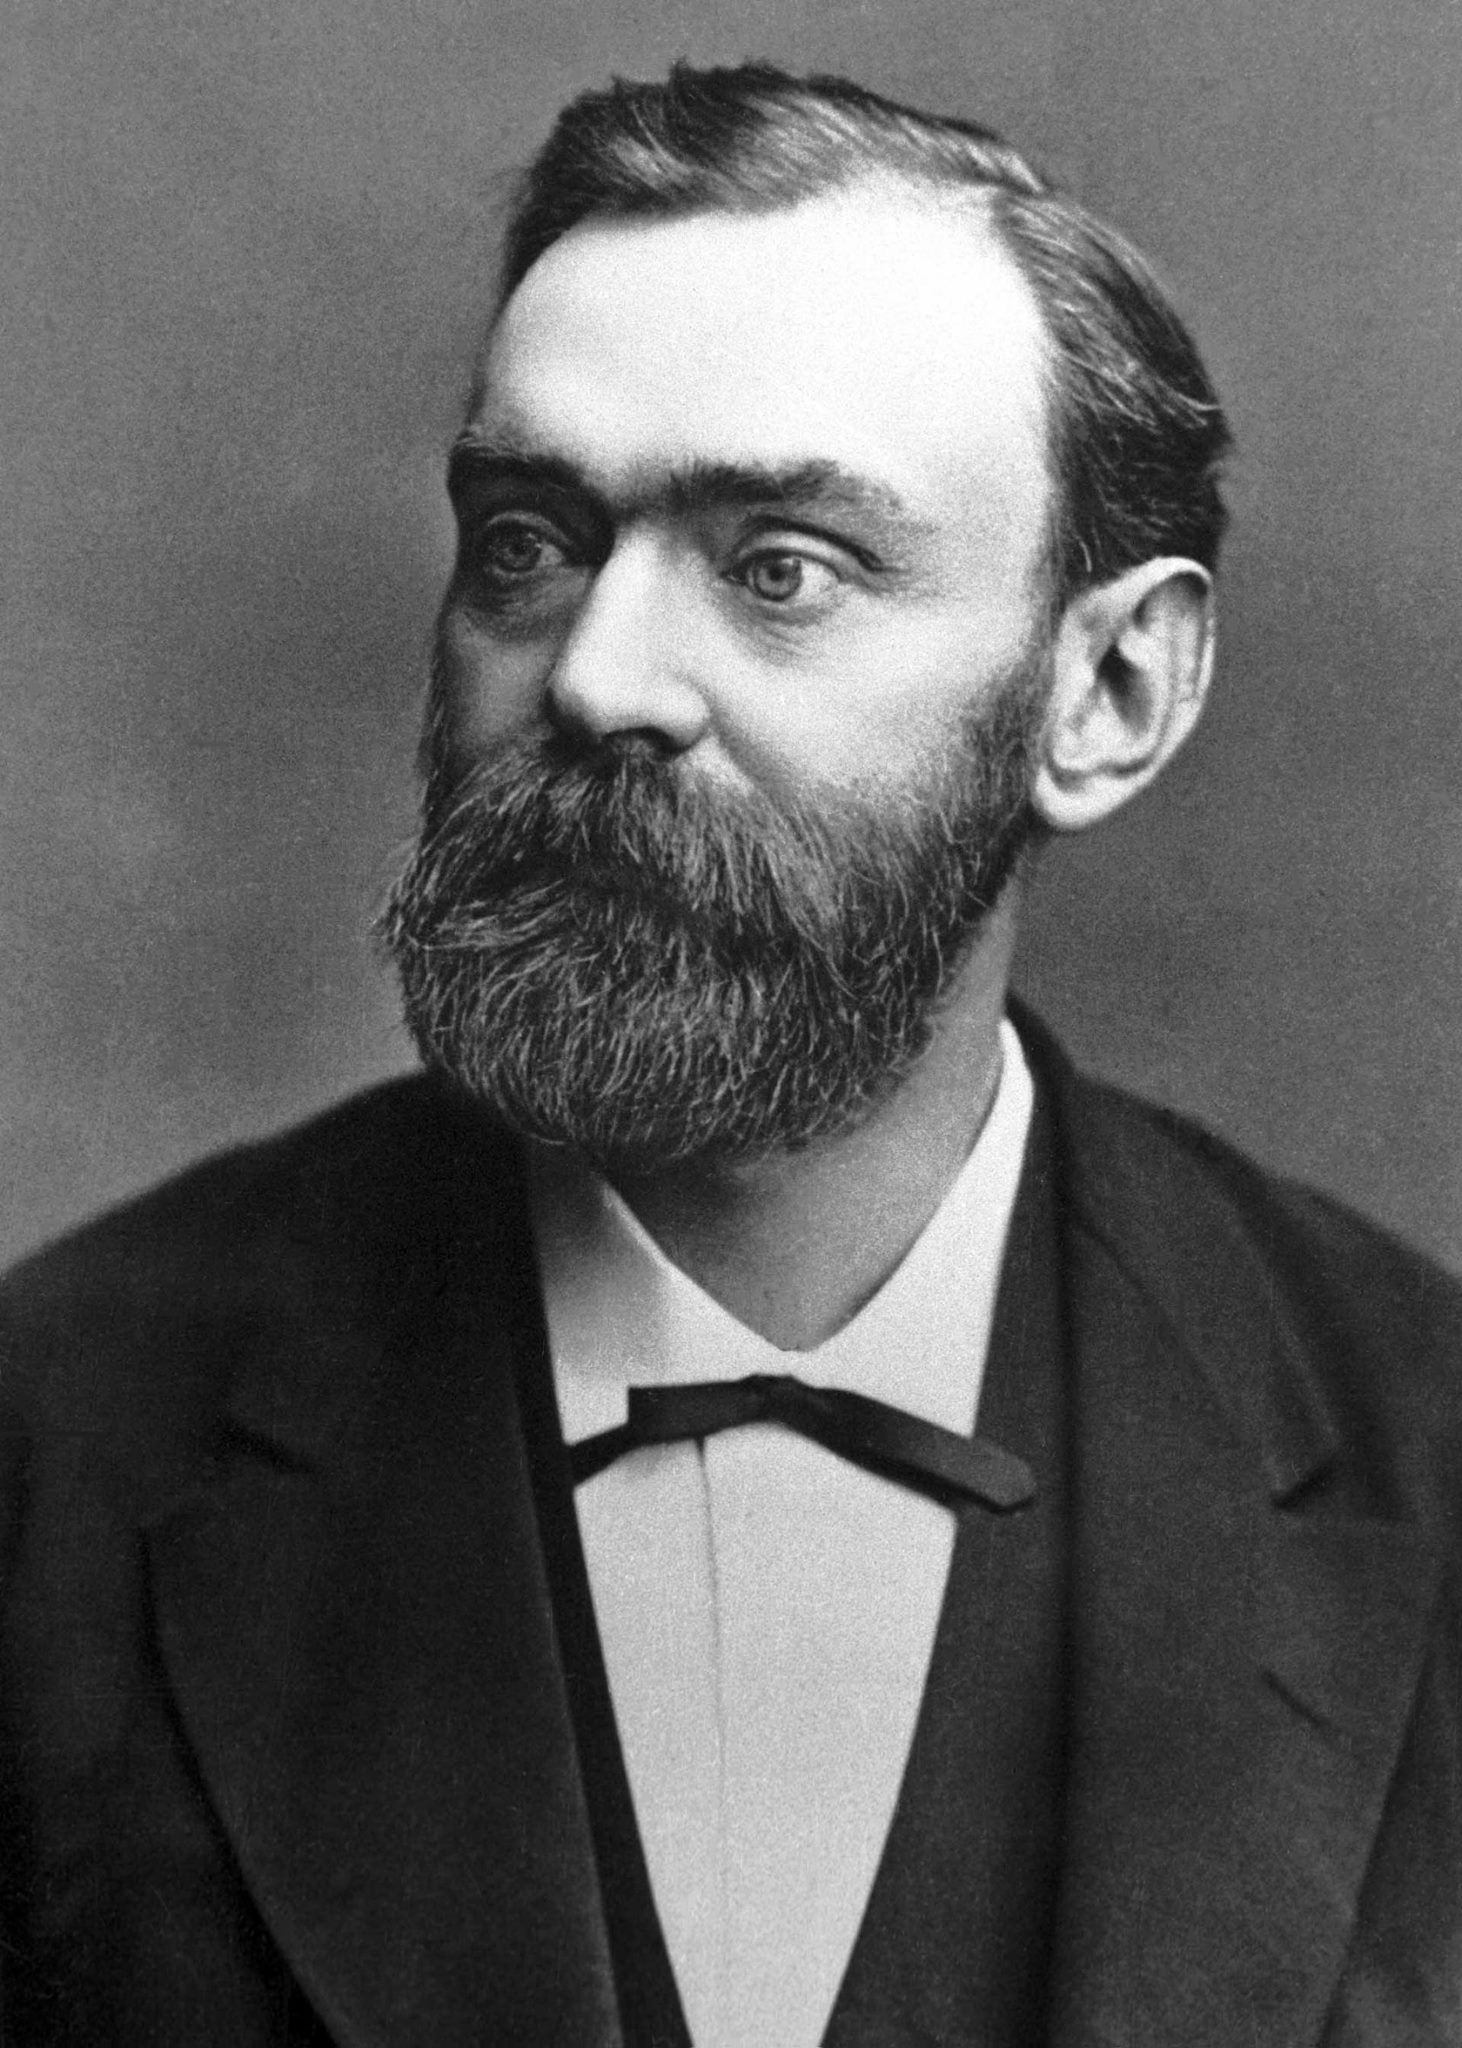
\includegraphics[width=\textwidth]{alfred.jpg}
        \caption{Alfred Nobel}
    \end{subfigure}
    \hfill%
    \begin{subfigure}[b]{0.33\textwidth}
        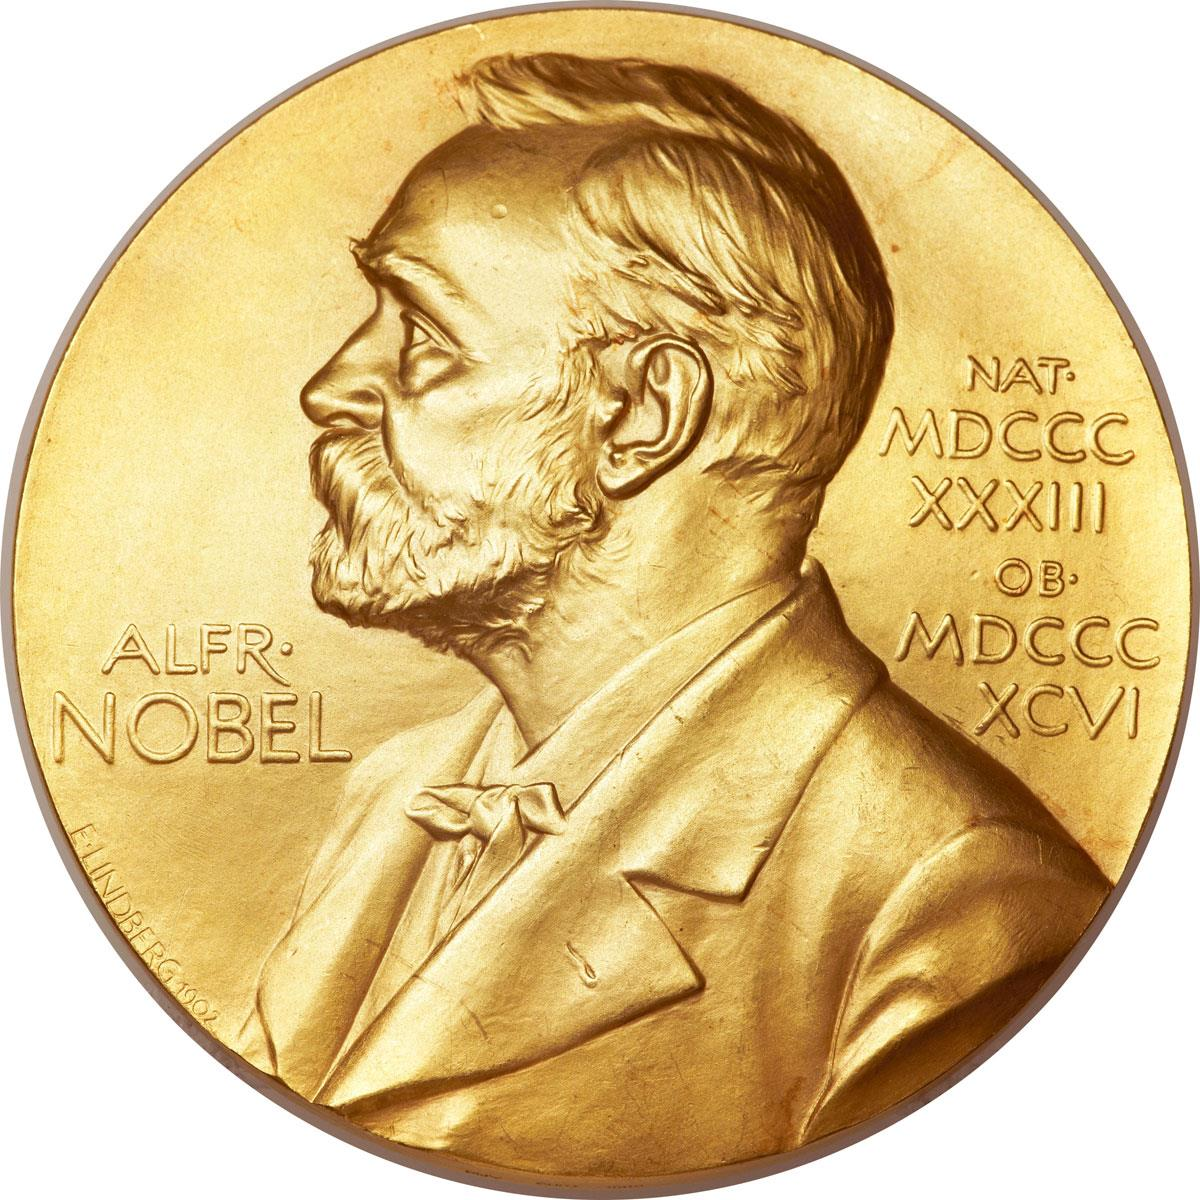
\includegraphics[width=\textwidth]{nobel.jpg}
        \caption{Alfred Nobel}
    \end{subfigure}
    \hfill
\end{figure}
\end{center}
\end{frame}



%%%%%%%%%%%%%%%%%%%%%%%%%%%%%%%%%%%%%%%%%%%%%%%%%%%%%%%%%%%%%%%%%%%%%%%%%%%%%%%%%%%%%%%%%%%%%%%
\subsection{The research question}
\begin{frame}
\frametitle{Our research question} 

\begin{center}
\textit{\Large Which European politicians have a high chance of
receiving a Nobel Prize?}
\end{center}



\end{frame}

\section{Methodology}
\begin{frame}
\frametitle{Methodology}
\framesubtitle{How we will tackle this problem}
\begin{enumerate}
\item<1-> Looking and finding available data
\item<2-> Collecting the data (SPARQL, scraping...)
\item<3-> Processing of data (training set \& research set (ToE))
\item<4-> Learning the model
\item<5-> Interpreting the results
\item<6-> Have a drink
\end{enumerate}
\end{frame}

\section{Data}
\subsection{Feature selection}
\begin{frame}
\frametitle{Feature selection}
\framesubtitle{Which features do we look for?}

\begin{enumerate}
\item<1-> Birth year \& -place
\item<2-> Ranking almamater
\item<3-> Number of publications/speeches
\item<4-> Popularity (likes on Facebook)
\item<5-> Nobel Prize: yes/no
\end{enumerate}

\end{frame}

\subsection{Data scheme}
\begin{frame}
\frametitle{Data scheme}
\framesubtitle{Our data sources: an overview}

\end{frame}

\subsection{Retrieved data}
\begin{frame}
\frametitle{Retrieved data}
\framesubtitle{What do we currently have?}

\end{frame}


\section{Data analysis}
\subsection{Outlier detection}
\section{Results}

\section{Conclusion}
\end{document}